\documentclass[DIV=calc, paper=a4, fontsize=11pt]{scrartcl}
\usepackage{makeidx}
\usepackage{graphicx}
\usepackage{flushend}

\usepackage{lmodern}
\usepackage[left=1.5cm,right=1.5cm,top=2.5cm,bottom=2cm]{geometry}
\usepackage{float}		
\bibliographystyle{plain} 
\pagestyle{plain} 
\pagenumbering{arabic}
\usepackage{fancyhdr} 	
\usepackage[T1]{fontenc}
\usepackage[utf8]{inputenc}
\usepackage[spanish]{babel}
\usepackage{hyperref}
\usepackage{graphicx}
\usepackage{siunitx}
\usepackage{lipsum}
\usepackage[protrusion=true,expansion=true]{microtype}
\usepackage{amsmath,amsfonts,amsthm}
\usepackage[svgnames]{xcolor}
\usepackage[svgnames]{xcolor}
\usepackage{booktabs}
\usepackage{fix-cm}
\usepackage{multicol}

\newenvironment{Figura}
  {\par\medskip\noindent\minipage{\linewidth}}
  {\endminipage\par\medskip}

\usepackage{sectsty}
\allsectionsfont{\usefont{OT1}{phv}{b}{n}}
\usepackage{fancyhdr}
\pagestyle{fancy}
\usepackage{lastpage}
\lhead{}
\chead{}
\rhead{}
\lfoot{}
\cfoot{}
\rfoot{\footnotesize Page \thepage\ of \pageref{LastPage}}
\renewcommand{\headrulewidth}{0.0pt}
\renewcommand{\footrulewidth}{0.4pt}
\usepackage{lettrine}
\newcommand{\initial}[1]{\lettrine[lines=3,lhang=0.3,nindent=0em]{
\color{DarkGoldenrod}{\textsf{#1}}}{}}
\usepackage{titling}
\newcommand{\HorRule}{\color{DarkGoldenrod} \rule{\linewidth}{1pt}}
\pretitle{\vspace{-120pt} \begin{flushleft} \HorRule \fontsize{22}{35} \usefont{OT1}{phv}{b}{n} \color{DarkRed} \selectfont}
\title{Determinación de la aceleración de la gravedad\\ %Aquí va el nombre de la práctica 
Práctica 1} %Numero de la práctica 
\posttitle{\par
\end{flushleft}
\vskip 0.5em}

\preauthor{\begin{flushleft}\large \lineskip 0.5em \usefont{OT1}{phv}{b}{sl} \color{DarkRed}}

\author{Misael Iván Macías Márquez\\
misaelmacias@ciencias.unam.mx}

\postauthor{\footnotesize \usefont{OT1}{phv}{m}{sl} \color{Black}

\vspace*{0.1cm} Facultad de Ciencias, UNAM

\par\end{flushleft}\HorRule}

\date{Viernes 25 de Febrero de 2022\\Semestre 2022-1}




\begin{document}

\maketitle


\begin{abstract}
\textbf{Resumen:} Se determinó la aceleración de la gravedad local haciendo uso de un péndulo armado con material casero. Se midió con un cronómetro el tempo de 20 oscilaciones, se utilizó el modelo del péndulo simple y se le aplicó el método de mínimos cuadrados con los datos obtenidos, la gravedad obtenida fue $(9.74 \pm 0.03)m/s^2$ dando una incertidumbre relativa del $0.3 \%$ y un error comparado con el valor real de $1.7$ veces la incertidumbre absoluta que al ser menor a $2$ se puede considerar un resultado satisfactorio.


\end{abstract}

\begin{multicols}{2}




\section*{Introducción}


Un péndulo simple se define como una partícula de masa $m$ suspendida de un punto $O$ por una cuerda de longitud $l$ y de masa despreciable, si la masa se lleva a un punto tal que la cuerda forme un ángulo $\theta$ con la vertical y se suelta, esta comenzará a oscilar entre el punto inicial y su simétrico respecto la vertical[1].


\begin{Figura}
    \centering
    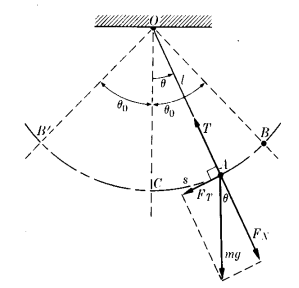
\includegraphics[width=0.7\textwidth]{pendulo.PNG}
    \captionof{figure}{Diagrama péndulo simple [1]}
    \label{fig}
\end{Figura}



Las fuerzas que actúa sobre la partícula son su peso $mg$ y la tensión $T$ y como se puede ver en la figura (1), la fuerza tangencial es $F_T = -mg \sin{\theta}$, la ecuación diferencial que describe este fenómeno es[1]:

\begin{equation}
    \frac{d^2 \theta}{d t^2} + \frac{g}{l} \sin{\theta} = 0
\end{equation}

\noindent pero suponiendo que el ángulo $\theta$ sea lo suficientemente pequeño para poder aproximar $\sin{\theta} \approx \theta$, se tiene[1]:

\begin{equation}
    \frac{d^2 \theta}{d t^2} + \frac{g}{l} \theta = 0
\end{equation}

\noindent lo que es muy parecido a la ecuación diferencial para el movimiento armónico simple con $\omega ^2 = \frac{g}{l}$ y dado que el período en función de la frecuencia angular es $T =\frac{ 2 \pi} {\omega}$, entonces $T= \frac{2\pi} {\sqrt{\frac{g}{l}}}$, o bien despejando $g$

\begin{equation}
    g = \frac{4 \pi^2 l}{T^2}
\end{equation}



\section*{Desarrollo experimental}




Como se puede ver en la figura 2, se colocó sobre un soporte metálico de una repisa para pared, sobre el soporte se introdujo una hoja de papel pegada a un pedazo de folder para mantenerse rígida, con ayuda de un transportador se marcaron los ángulos $\pm \theta$, se ajusto el hilo cáñamo sobre el soporte y en el extremo suelto del hilo se sujetó un tornillo de masa $m$ de tal forma que su eje de simetría vertical coincidiera con la vertical del péndulo.


\begin{Figura}
    \centering
    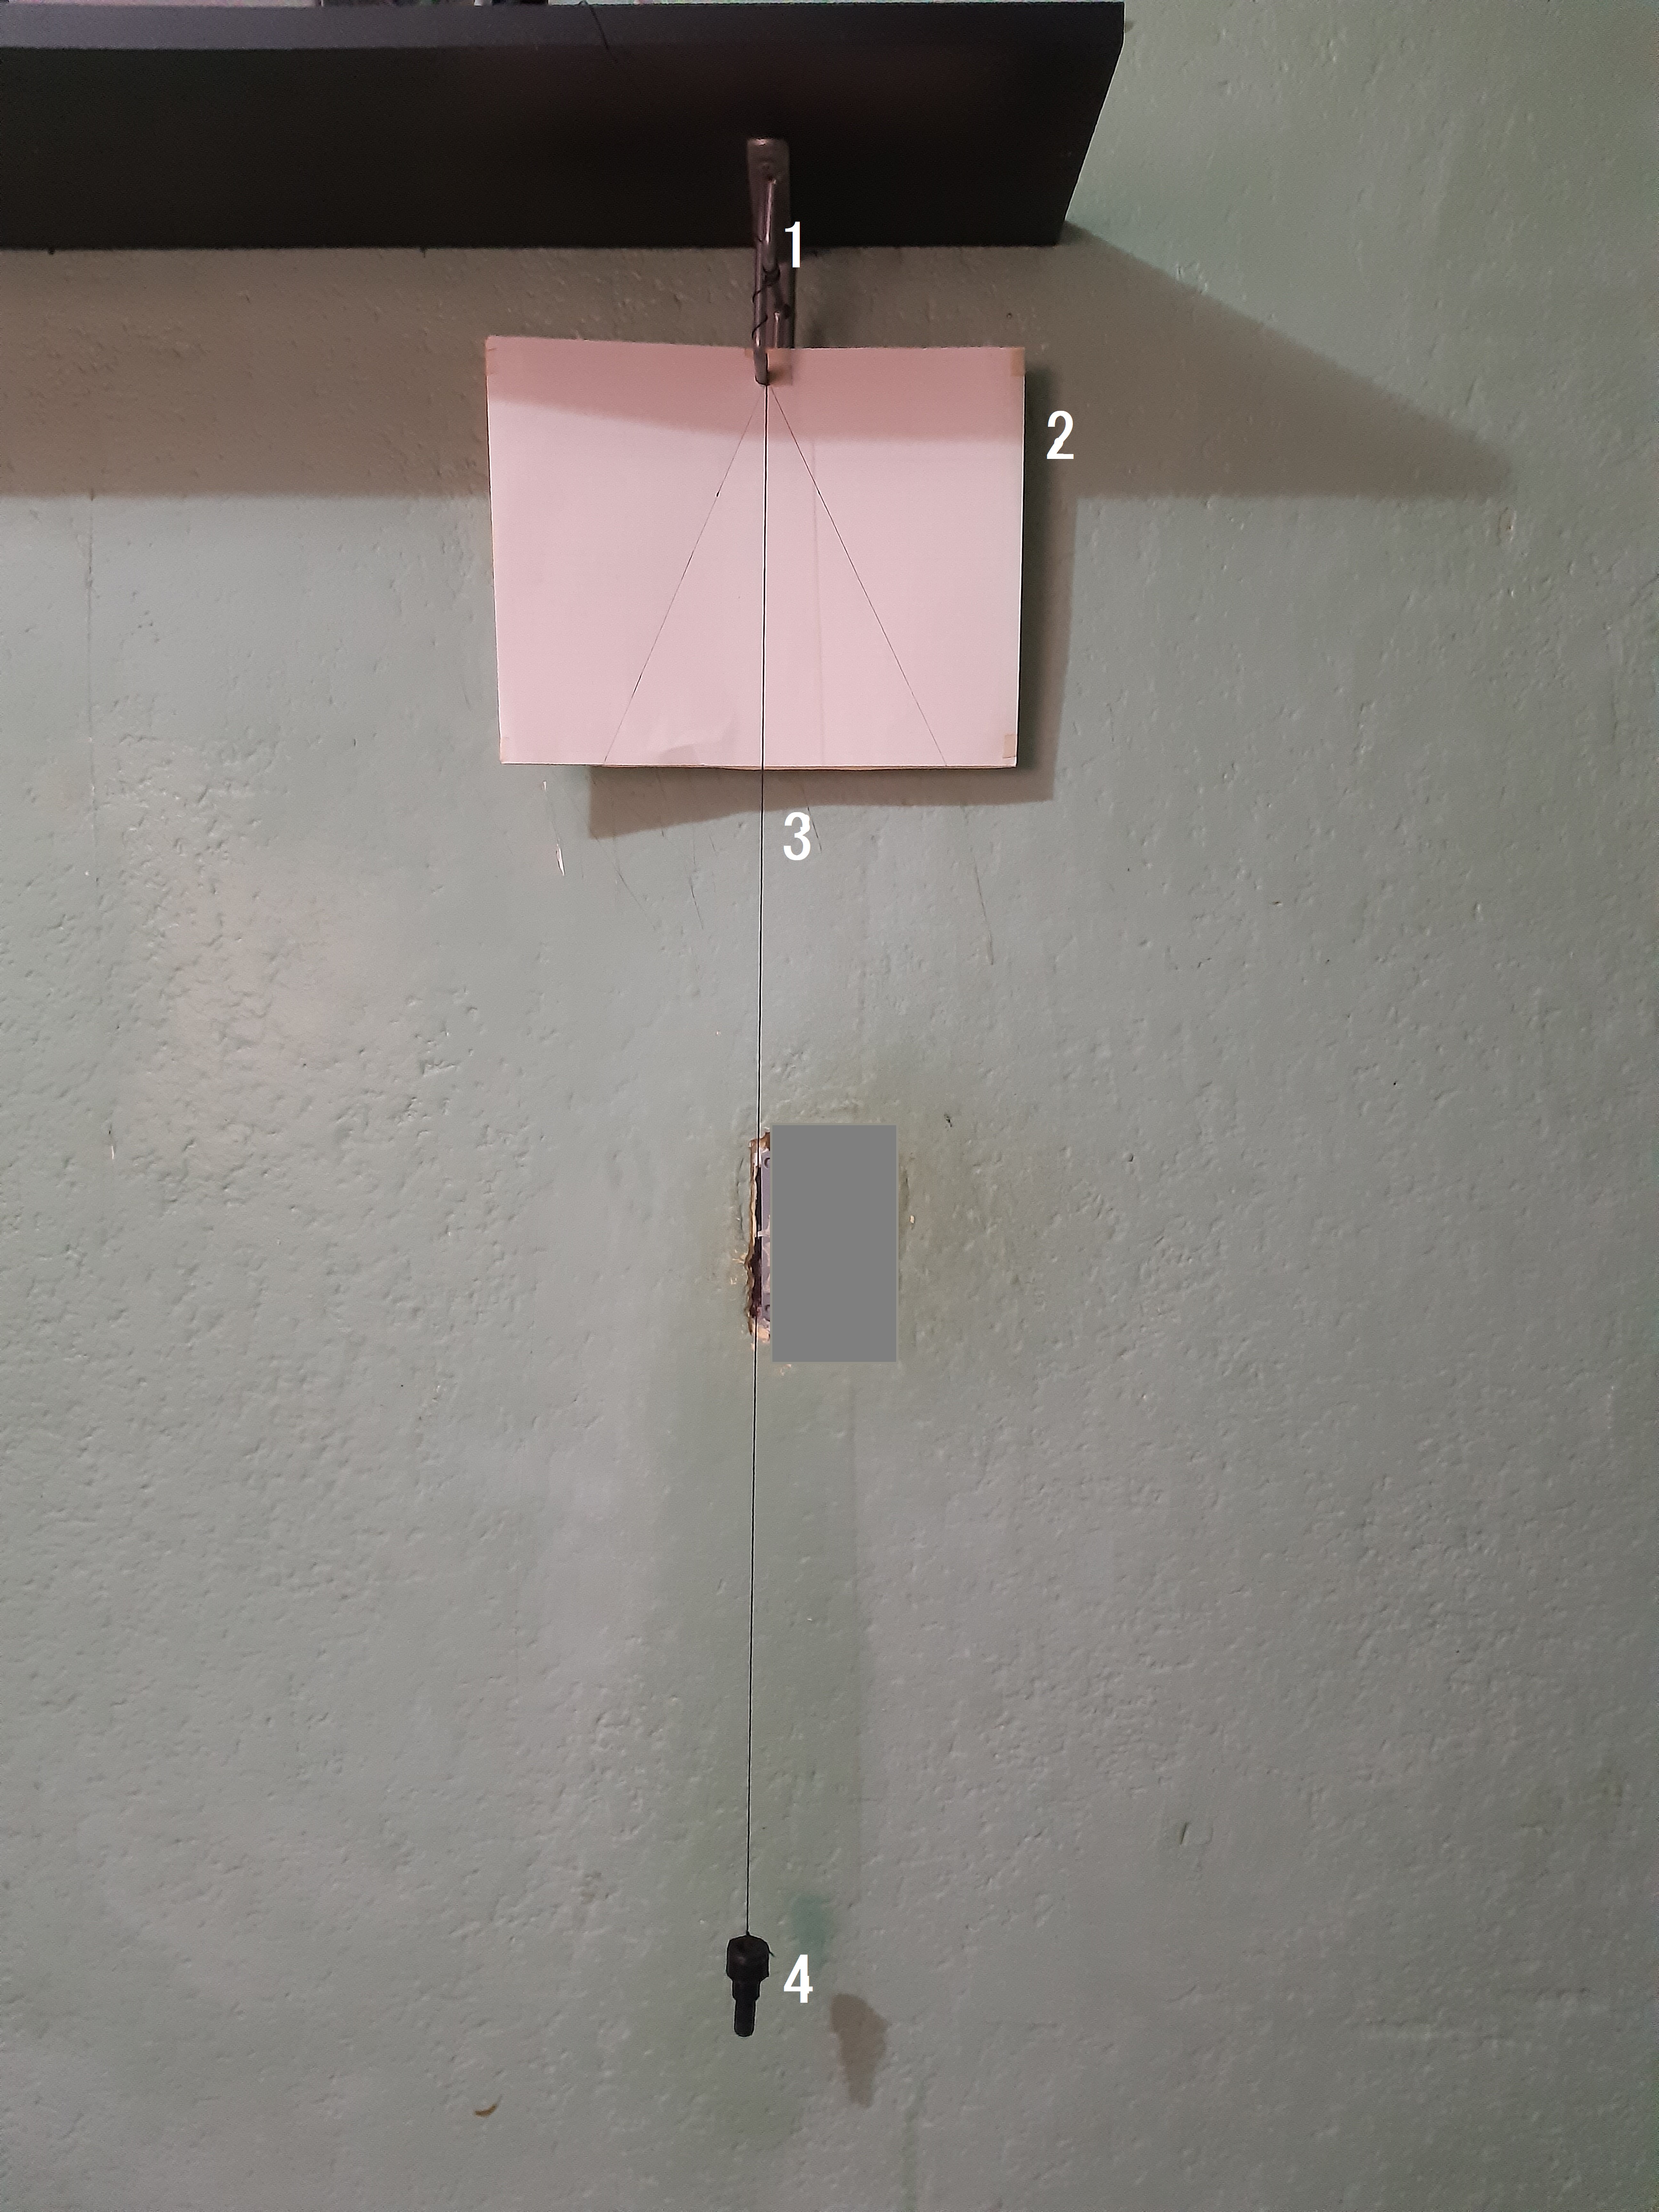
\includegraphics[width=0.9\textwidth]{20220219_161348.jpg}
    \captionof{figure}{Arreglo Experimental: (1) Soporte de repisa,(2) Papel con marca de ángulos, (3) Hilo cáñamo, (4) Tornillo}
    \label{fig}
\end{Figura}

Antes de que el péndulo comenzara a oscilar,Primero se midió el tiempo de reacción con el cronómetro, para esto se realizaron 10 intentos de detener el cronómetro justo a los 3 segundos de haberlo iniciado y de estos se tomo el promedio de la diferencia como el tiempo de reacción.

 Con una cinta métrica se midió la longitud del hilo desde su origen hasta el centro de masa aproximado del tornillo y después se realizaron 5 mediciones de tiempo para 20 oscilaciones ($T$) colocando el tornillo en el ángulo $\theta$ de lado derecho. Esto se repitió para las longitudes de $0.1 m$, $0.2 m$, $0.3 m$, $0.4 m$, $0.5 m$, $0.6 m$, $0.7 m$, $0.8 m$, $0.9 m$ y $1m$.

\section*{Resultados y Análisis}



Los valores que tomaron las variables descritas en el desarrollo experimental a excepción de los  tiempos, períodos y longitudes (ver Apéndice).

\begin{equation*}
    \theta = (25 \pm 1) ^{\circ}C \hspace{1cm} m = (76 \pm 1)g
\end{equation*}

Las longitudes de los péndulos se reportaron con una incertidumbre del $5\%$ debido a problemas de definición tanto del origen del péndulo como del centro de masa del tornillo.

En el caso de los tiempos de reacción (ver apéndice), la incertidumbre absoluta está dada por tanto el tiempo de reacción $\sigma_{def} = 0.092 s$ y la escala mínima del cronómetro $\sigma_{ap} = 0.001s$ por lo que la incertidumbre absoluta es:

\begin{equation*}
    \delta t = \sqrt{\sigma_{def}^2 + \sigma_{ap}^2} = 0.092 s
\end{equation*}

\noindent y dado que en este tiempo sucedieron 20 periodos, propagando la incertidumbre tenemos que:

\begin{equation*}
    \delta T = \frac{\delta t}{20} = 0.005 s
 \end{equation*}
 
 Entonces tomando el tiempo promedio para cada péndulo y sumando por cuadraturas cada incertidumbre presente, se llega a que la incertidumbre de los promedios de periodos es $\delta \hat{T} = 0.006$.

Para determinar $g$ se linealizó la ecuación (3) de la siguiente forma

\begin{equation}
    l = \left(\frac{g}{4\pi^2}\right) \hat{T}^2
\end{equation}

\noindent por lo que al propagar la incertidumbre de $\hat{T}^2$ tenemos una relativa de $1.2\%$, usando el método de mínimos cuadrados se puede determinar la pendiente 

\begin{equation*}
    \frac{g}{4 \pi^2}
\end{equation*}

Los datos graficados en la figura 3 se pueden consultar en los apéndices.

$\vspace{0.1cm}$


\begin{Figura}
    \centering
    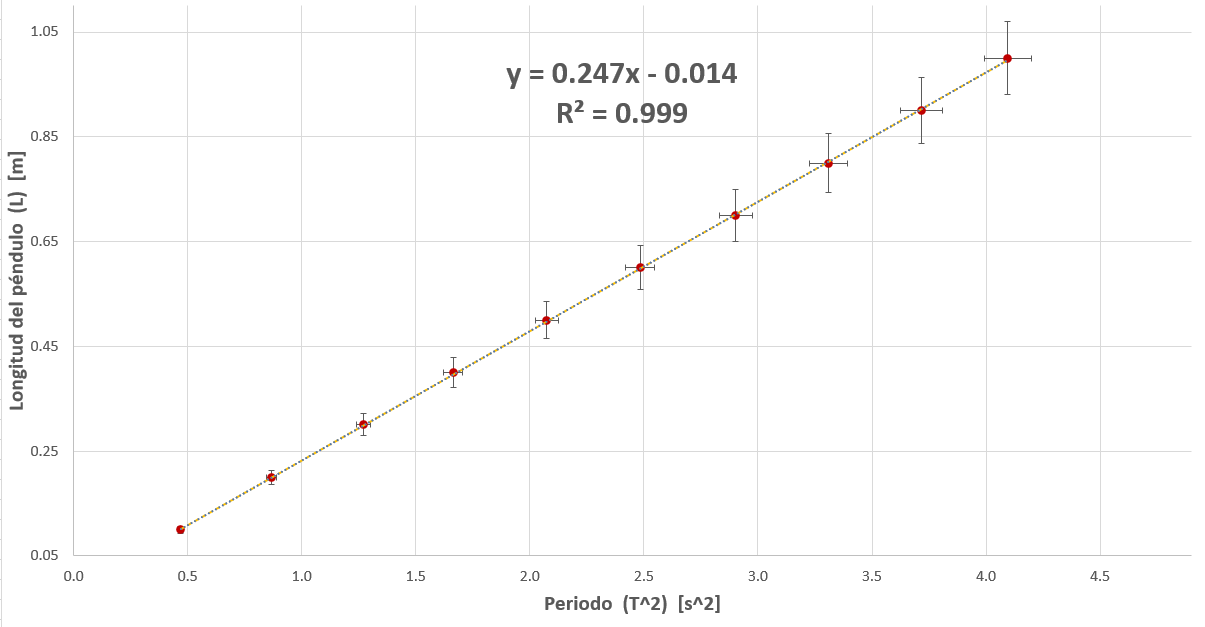
\includegraphics[width=1\textwidth]{grafica gravedad.PNG}
    \captionof{figure}{Gráfica del ajuste por mínimos cuadrados y datos de mediciones linealizadas según la ecuación (4)}
    \label{fig}
\end{Figura}

La pendiente y ordenada al origen resultantes son:

\begin{equation*}
    m = (0.247 \pm 0.001) m/s^2
\end{equation*}

\begin{equation*}
    b = (0.014 \pm 0.02)\footnote{Nótese que el 0 entra en este intervalo} m
\end{equation*}

\noindent por lo tanto despejando a $g$ y propagando la incertidumbre,

\begin{equation*}
    g= 4\pi^2 m
\end{equation*}

\begin{equation*}
    \delta g =  4\pi^2 \delta m
\end{equation*}

\noindent obtenemos un valor para la aceleración de la gravedad de:

\begin{equation*}
    g = (9.74 \pm 0.03) m/s^2
\end{equation*}





\section*{Conclusiones}

El arreglo experimental usado aunque mostró algunas dificultades, considero fue suficiente para tener una buena medición de la aceleración de la gravedad ya que el error del valor real\footnote{Calculado con la ecuación (4) presente en [3] usando datos recabados en Google Maps} y la medición fue de $0.05 m/s^2$ o $1.7$ veces la incertidumbre absoluta de $g$ medida, además de tener una incertidumbre relativa de $0.3\%$, por lo tanto el resultado es satisfactorio.
  
\begin{thebibliography}{99}
\bibitem{1} Alonso, Marcelo y Edward J. Finn. FISICA Vol I: MECANICA. Ciudad de México: Fondo Educativo Interamericano, 1971.

\bibitem{2} Oda, Berta. Introducción al análisis gráfico de datos experimentales. 3a ed. Ciudad de México: las prensas de ciencias, 2017.

\bibitem{3} Ramos, R., et al., ESTUDIO GEOESTADÍSTICO PARA OBTENER LA GRAVEDAD LOCAL, PENDIENTE Y CÁLCULO HIDROLÓGICO DE LAS BARRANCAS XALTELULCO, TEPELONCOCONE, TENEPANCO, COLORADA Y QUIMICHULE DEL VOLCÁN POPOCATÉPETL. Puebla, 2012. 


\end{thebibliography}




\section*{Apéndices}

\subsection*{Notación}

\noindent $x_i$, $y_i$ = mediciones realizadas

\noindent $N$ = número de repeticiones 

\noindent $m$ = pendiente (usada en el método de mínimos cuadrados)

\noindent $b$ = ordenada al origen (usada en el método de mínimos cuadrados)

\noindent $\hat{x}$ = promedio de mediciones $x_i$

\noindent $S_x$ = desviación estándar para los valores $x_i$

\noindent $\sigma_{est}$ = incertidumbre estadística

\noindent $\sigma_{ap}$ = incertidumbre de apreciación

\noindent $\sigma_{def}$ = incertidumbre de definición

\noindent $\delta$ = incertidumbre absoluta (obtenida por suma por cuadraturas de las incertidumbres encontradas)


\begin{equation*}
    S_x = \sqrt{\frac{\sum_{i=1}^{N} (x_i- \hat{x})^2}{N-1}}
\end{equation*}

\begin{equation*}
    \sigma_{est} = \frac{S_x}{\sqrt{N}}
\end{equation*}

\begin{equation*}
    \chi ^2 = \sum_{i=1}^{N} [y_i - (m x_i + b)]
\end{equation*}

\begin{equation*}
    \chi _N =\sqrt{\frac{\chi^2}{N-2}}
\end{equation*}

\begin{equation*}
    \Delta = N \sum_{i=1}^{N} x_{i}^{2} - (\sum_{i=1}^{N}x_i)^2
\end{equation*}


\subsection*{Tiempos de reacción}

\begin{tabular}{||c| c||} 
 \hline
 tiempo de reacción [s] & diferencia  [s] \\ [0.5ex] 
 \hline\hline
 3.010 & 0.010  \\ 
 3.021 &  0.021 \\
 2.770 & 0.230 \\
 3.094 &  0.094\\
 2.825 &  0.175\\
 2.976 & 0.024\\
 3.118 & 0.118\\
 3.103 & 0.103\\
 2.905 & 0.095\\
 3.024 & 0.024\\
  [1ex] 
 \hline
\end{tabular}

\begin{equation*}
    \hat{x} = 0.089s \hspace{0.3cm} S_x = 0.073 \hspace{0.3cm} \sigma_{est} = 0.023 \hspace{0.3cm} \delta = 0.092
\end{equation*}



\subsection*{Tabla 1: Tiempos Medidos}







\centering

\begin{tabular}{||c| c||} 
 \hline
 tiempo (t) $\pm$ 0.089 [s] & período (T) \pm 0.005 [s] \\ [0.5ex] 
 20 oscilaciones &  \\
 \hline\hline
 40.418 & 2.021  \\ 
 40.442 & 2.022  \\
 40.427 & 2.021 \\
 40.593 & 2.030 \\
 40.477 & 2.024 \\
  [1ex] 
 \hline
\end{tabular}

\caption{Tabla 2: péndulo de $(1 \pm 0.05)m$ }

\begin{equation*}
    \hat{T} = 2.024s \hspace{0.3cm} S_T= 0.004s \hspace{0.3cm} \sigma_{est} = 0.002s \hspace{0.3cm} \sigma_{ap} = 0.001s 
\end{equation*}

$\vspace{1cm}$

\begin{tabular}{||c| c||} 
 \hline
 tiempo (t) \pm 0.089 [s] & período (T) \pm 0.005 [s] \\ [0.5ex] 
 20 oscilaciones &  \\
 \hline\hline
 38.555 & 1.928  \\ 
 38.395 & 1.920  \\
 38.545 & 1.927 \\
 38.633 & 1.932 \\
 38.694 & 1.935 \\
  [1ex] 
 \hline
\end{tabular}

\caption{Tabla 3: péndulo de $(0.9 \pm 0.045 )m$}

\begin{equation*}
    \hat{T} = 1.928s \hspace{0.3cm} S_T= 0.006s \hspace{0.3cm} \sigma_{est} = 0.003s \hspace{0.3cm} \sigma_{ap} = 0.001s 
\end{equation*}



$\vspace{1cm}$

\begin{tabular}{||c| c||} 
 \hline
 tiempo (t) \pm 0.089 [s] & período (T) \pm 0.005 [s] \\ [0.5ex] 
 20 oscilaciones &  \\
 \hline\hline
 36.361 & 1.808  \\ 
 36.450 & 1.823  \\
 36.239 & 1.812 \\
 36.467 & 1.823 \\
 36.407 & 1.820 \\
  [1ex] 
 \hline
\end{tabular}

\caption{Tabla 4: péndulo de $(0.8 \pm 0.04)m$}

\begin{equation*}
    \hat{T} = 1.819s \hspace{0.3cm}S_T= 0.005s \hspace{0.3cm} \sigma_{est} = 0.002s \hspace{0.3cm} \sigma_{ap} = 0.001s 
\end{equation*}

$\vspace{1cm}$

\begin{tabular}{||c| c||} 
 \hline
 tiempo (t) \pm 0.089 [s] & período (T) \pm 0.005 [s] \\ [0.5ex] 
 20 oscilaciones &  \\
 \hline\hline
 34.192 & 1.710  \\ 
 34.088 & 1.704  \\
 33.925 & 1.696 \\
 34.119 & 1.706 \\
 34.020 & 1.701 \\
  [1ex] 
 \hline
\end{tabular}

\caption{Tabla 5: péndulo de $(0.7 \pm 0.035)m$}

\begin{equation*}
    \hat{T} = 1.703s \hspace{0.3cm}S_T= 0.005s \hspace{0.3cm} \sigma_{est} = 0.002s \hspace{0.3cm} \sigma_{ap} = 0.001s 
\end{equation*}

$\vspace{1cm}$

\begin{tabular}{||c| c||} 
 \hline
 tiempo (t) \pm 0.089 [s] & período (T) \pm 0.005 [s] \\ [0.5ex] 
 20 oscilaciones &  \\
 \hline\hline
 31.496 & 1.575  \\ 
 31.450 & 1.573  \\
 31.559 & 1.578 \\
 31.603 & 1.580 \\
 31.477 & 1.574 \\
  [1ex] 
 \hline
\end{tabular}

\caption{Tabla 6: péndulo de $(0.6 \pm 0.03)m$}

\begin{equation*}
    \hat{T} = 1.576s \hspace{0.3cm}S_T= 0.003s \hspace{0.3cm} \sigma_{est} = 0.001s \hspace{0.3cm} \sigma_{ap} = 0.001s 
\end{equation*}

$\vspace{1cm}$

\begin{tabular}{||c| c||} 
 \hline
 tiempo (t) \pm 0.089 [s] & período (T) \pm 0.005 [s] \\ [0.5ex] 
 20 oscilaciones &  \\
 \hline\hline
 28.718 & 1.436  \\ 
 28.873 & 1.444  \\
 28.807 & 1.440 \\
 28.905 & 1.445 \\
 28.723 & 1.436 \\
  [1ex] 
 \hline
\end{tabular}

\caption{Tabla 6: péndulo de $(0.5\pm 0.25 )m$}

\begin{equation*}
    \hat{T} = 1.440s \hspace{0.3cm} S_T= 0.004s \hspace{0.3cm} \sigma_{est} = 0.002s \hspace{0.3cm} \sigma_{ap} = 0.001s 
\end{equation*}

$\vspace{1cm}$

\begin{tabular}{||c| c||} 
 \hline
 tiempo (t) \pm 0.089 [s] & período (T) \pm 0.005 [s] \\ [0.5ex] 
 20 oscilaciones &  \\
 \hline\hline
 25.785 & 1.289  \\ 
 25.901 & 1.295  \\
 25.928 & 1.296 \\
 25.708 & 1.285 \\
 25.671 & 1.284 \\
  [1ex] 
 \hline
\end{tabular}

\caption{Tabla 7: péndulo de $(0.4\pm 0.02) m$}

\begin{equation*}
    \hat{T} = 1.290s \hspace{0.3cm} S_T= 0.006s \hspace{0.3cm} \sigma_{est} = 0.003s \hspace{0.3cm} \sigma_{ap} = 0.001s 
\end{equation*}

$\vspace{1cm}$

\begin{tabular}{||c| c||} 
 \hline
 tiempo (t) \pm 0.089 [s] & período (T) \pm 0.005 [s] \\ [0.5ex] 
 20 oscilaciones &  \\
 \hline\hline
 22.588 & 1.129  \\ 
 22.561 & 1.128  \\
 22.482 & 1.124 \\
 22.493 & 1.125 \\
 22.610 & 1.131 \\
  [1ex] 
 \hline
\end{tabular}

\caption{Tabla 8: péndulo de $(0.3\pm 0.015) m$}

\begin{equation*}
   \hat{T} = 1.127s \hspace{0.3cm} S_T= 0.003s \hspace{0.3cm} \sigma_{est} = 0.001s \hspace{0.3cm} \sigma_{ap} = 0.001s 
\end{equation*}

$\vspace{1cm}$

\begin{tabular}{||c| c||} 
 \hline
 tiempo (t) \pm 0.089 [s] & período (T) \pm 0.005 [s] \\ [0.5ex] 
 20 oscilaciones &  \\
 \hline\hline
 18.525 & 0.926  \\ 
 18.631 & 0.932  \\
 18.726 & 0.936 \\
 18.628 & 0.931 \\
 18.661 & 0.933 \\
  [1ex] 
 \hline
\end{tabular}

\caption{Tabla 9: péndulo de $(0.2\pm 0.01 )m$}

\begin{equation*}
    \hat{T} = 0.932s \hspace{0.3cm} S_T= 0.004s \hspace{0.3cm} \sigma_{est} = 0.002s \hspace{0.3cm} \sigma_{ap} = 0.001s 
\end{equation*}

$\vspace{1cm}$

\begin{tabular}{||c| c||} 
 \hline
 tiempo (t) \pm 0.089 [s] & período (T) \pm 0.005 [s] \\ [0.5ex] 
 20 oscilaciones &  \\
 \hline\hline
 13.549 & 0.677  \\ 
 13.621 & 0.681  \\
 13.774 & 0.689 \\
 13.797 & 0.690 \\
 13.825 & 0.691 \\
  [1ex] 
 \hline
\end{tabular}

\caption{Tabla 10: péndulo de $(0.1\pm 0.005) m$}

\begin{equation*}
    \hat{T} = 0.686s \hspace{0.3cm} S_T= 0.006s \hspace{0.3cm} \sigma_{est} = 0.003s \hspace{0.3cm} \sigma_{ap} = 0.001s 
\end{equation*}



\subsection*{Ajuste por Mínimos Cuadrados}

Al linealizar los datos tenemos que los puntos a ajustar son:

$\vspace{0.3cm}$

\begin{tabular}{||c| c||} 
 \hline
 período [T^2] \pm 1.2\% [s^2] & longitud (l) \pm 5\%  [m] \\ [0.5ex] 
 \hline\hline
  $4.095 $ & $0.1 $  \\ 
 $3.718$ & $ 0.2$ \\
 $3.310 $ & $0.3 $ \\
 $2.902 $ &  $0.4 $\\
 $2.483 $ &  $0.5$\\
 $2.074 $ & $0.6$\\
 $1.664 $ & $0.7 $\\
 $1.271 $ & $0.8 $\\
 $0.868 $ & $0.9 $\\
 $0.470 $ & $1 $\\
  [1ex] 
 \hline
\end{tabular}

\caption{tabla 11: puntos ajustados por mínimos cuadrados}

El ajuste de este método se puede realizar fácilmente en Excel usando el comando 'ESTIMACION.LINEAL()' aunque las formulas y sus correspondientes incertidumbres [2] se muestran a continuación:

\begin{equation*}
    m = \frac{N\sum T_{i}^{2} l_i - \sum T_{i}^{2} \sum l_{i}^{2}}{N \sum (T_{i}^{2})^2 - (\sum T_{i}^{2})^2}
\end{equation*}

\begin{equation*}
    b = \frac{\sum (T_{i}^{2})^2 \sum l_{i} - \sum T_{i}^{2} \sum T_{i}^{2} l_{i}}{N \sum (T_{i}^{2})^2 - (\sum T_{i}^{2})^2}
\end{equation*}

con incertidumbres

\begin{equation*}
    \delta m =  \chi_N \sqrt{\frac{\sum (T_{i}^{2})^2}{\Delta}}
\end{equation*}

\begin{equation*}
    \delta b = \chi_N \sqrt{\frac{N}{\Delta}}
\end{equation*}


\subsection*{Calculo del valor real de la aceleración de gravedad Local}


La ecuación que nos permite conocer de forma precisa (con una incertidumbre relativa del $0.1\%$) la aceleración de la gravedad  según la latitud y altitud es [3]:

\begin{equation}
    g = g_e (1 +f_1 \sin^2{\theta} + f_2 \sin^2{(2\theta)}) - \num{3.086 e -6} h
\end{equation}

donde 

\begin{itemize}
    \item $g_e$ es la gravedad en el ecuador ($9.780318 m/s^2$)
    
        \item $f_1$ es el aplastamiento gravitacional ($0.005302$)
    
    \item $\theta$ es la latitud en grados ($19.28 ^{\circ}$)
    
    \item $f_2$ ($0.000006$)
    
    \item $h$ es la altitud sobre el nivel del mar en metros ($2230$)

\end{itemize}

\noindent por lo que sustituyendo obtenemos una gravedad local de:

\begin{equation*}
    g = (9.79 \pm 0.01)  m/s^2
\end{equation*}


 



\end{multicols}
\end{document}